%%% LaTeX Template: Article/Thesis/etc. with colored headings and special fonts
%%%
%%% Source: http://www.howtotex.com/
%%% Feel free to distribute this template, but please keep to referal to http://www.howtotex.com/ here.
%%% February 2011
%%%
%%% Last updated September 2018 by CDM

%%%  Preamble
\documentclass[11pt,letterpaper]{article}
\usepackage[margin=1.0in]{geometry}
\usepackage[T1]{fontenc}
\usepackage[bitstream-charter]{mathdesign}
\usepackage[latin1]{inputenc}					
\usepackage{amsmath}						
\usepackage{xcolor}
\usepackage{cite}
\usepackage{hyphenat}
\usepackage{graphicx}
\usepackage{float}
\usepackage{subfigure}
\usepackage{sectsty}
\usepackage[compact]{titlesec} 
\usepackage[tablegrid]{vhistory}
\allsectionsfont{\color{accentcolor}\scshape\selectfont}

%%% Definitions
\definecolor{accentcolor}{rgb}{0.0,0.0,0.5} 
\newcommand{\teamname}{Resonance}
\newcommand{\productname}{Project LTunes}
\newcommand{\coursename}{CSE 4316: Senior Design II}
\newcommand{\semester}{Spring 2020}
\newcommand{\docname}{Project Charter}
\newcommand{\department}{Department of Computer Science \& Engineering}
\newcommand{\university}{The University of Texas at Arlington}
\newcommand{\authors}{Amir Dhungana \\ Anish Yonjan \\ Nikhil Purohit \\ Rabinson Shrestha \\ Raul Jimenez \\ Roberto Torres}

%%% Headers and footers
\usepackage{fancyhdr}
	\pagestyle{fancy}						% Enabling the custom headers/footers
\usepackage{lastpage}	
	% Header (empty)
	\lhead{}
	\chead{}
	\rhead{}
	% Footer
	\lfoot{\footnotesize \teamname \ - \semester}
	\cfoot{}
	\rfoot{\footnotesize page \thepage\ of \pageref{LastPage}}	% "Page 1 of 2"
	\renewcommand{\headrulewidth}{0.0pt}
	\renewcommand{\footrulewidth}{0.4pt}

%%% Change the abstract environment
\usepackage[runin]{abstract}			% runin option for a run-in title
%\setlength\absleftindent{30pt}			% left margin
%\setlength\absrightindent{30pt}		% right margin
\abslabeldelim{\quad}	
\setlength{\abstitleskip}{-10pt}
\renewcommand{\abstractname}{}
\renewcommand{\abstracttextfont}{\color{accentcolor} \small \slshape}	% slanted text

%%% Start of the document
\begin{document}

%%% Cover sheet
{\centering \huge \color{accentcolor} \sc \textbf{\department \\ \university} \par}
\vspace{1 in}
{\centering \huge \color{accentcolor} \sc \textbf{\docname \\ \coursename \\ \semester} \par}
\vspace{0.5 in}
\begin{figure}[h!]
	\centering
   	
\includegraphics[width=0.60\textwidth]{images/logo.png}
\end{figure}
\vspace{0.5 in}
{\centering \huge \color{accentcolor} \sc \textbf{\teamname \\ \productname} \par}
\vspace{0.5 in}
{\centering \large \sc \textbf{\authors} \par}
\newpage


%\vspace{1 in}
%\centerline{January 13th, 2012}
%\newpage

%%% Revision History
\begin{versionhistory}
  	\vhEntry{0.1}{10.01.2019}{GH}{document creation}
  	\vhEntry{0.2}{10.05.2019}{AT|GH}{complete draft}
  	\vhEntry{0.3}{10.12.2019}{AT|GH}{release candidate 1}
  	\vhEntry{1.0}{10.20.2019}{AT|GH|CB}{official release}
  	\vhEntry{1.1}{10.31.2019}{AL}{added customer change requests}
  	\vhEntry{2.0}{05.10.2010}{RT}{Updated with changes due to Covid-19}
\end{versionhistory}
\newpage

%%% Table of contents
\tableofcontents
\newpage

%%% List of figures and tables (optional)
\listoffigures
%\listoftables
\newpage
\setcounter{table}{0}

%%% Agile project charter sections
\section{Vision}
To create an electronic musical interface using visible lasers for the handicapped as well as enthusiasts.

\section{Mission}
Our mission is to design and create a laser-based instrument that produces tonal sounds, while also functioning as a MIDI device for versatility. The ‘laser synth’ is going to be portable and based on a Raspberry Pi. The laser diodes emit laser signals which is detected by the system, any interference to it will be detected giving a signal for the audio output. The instrument will be easy to use, so that even children can play the device at ease, while also learning about sounds.

\section{Success Criteria}
In the first 2 sprint cycles, we expect the following success indicators to be observed:
•	Complete initial research and have a general layout of how the design is going to look like
•	Division of labor all planned out and everyone has proper assigned tasks to work on

Within the first 3 months, we expect following success indicators to be observed:
•	Prototypes of the device are functional

Within 7 months, we expect the following success indicators to be observed:
•	Final device is complete and working well
•	Additional features are added as needed

\newpage

%%% Remaining project charter sections
\section{Background}
An in-depth explanation of the problem, including the "business case". What is wrong with the status-quo or what opportunity exists that justifies undertaking this project (expanding upon the vision statement)?

If you have a clear customer or sponsor, why do they want you to work on this? What is the existing relationship, if any, between the development team and the customer? This section should occupy 1/2 - 1 full page.

//

Most instruments require serious skill and strength to use properly in order to get tones out of it. Whether it is a plucked instrument like a harp or a guitar, or even a violin, there are specific techniques on how it can be played. On top of it all, people with medical conditions or disabilities like carpal tunnel or arthritis cannot play most instruments due to the force required. On top of it all, in an increasingly digital world where everything is accessible at our finger tips, versatility is everything. Even, music these days is getting more and more complex,  which often involves several instruments and relies on their syncopation to create a groove and melody that drives the song. Having some sort of instrument that is versatile, yet easy to use solves the key problem here. In essence, some type of MIDI device (at the core) provides us the greatest versatility, all the while keeping user inputs the same. Lasers come into play here as they can be used for detecting input, as there are two states: when the laser is blocked, or when the laser is not blocked. With those two states we can associate a note being triggered with when the laser is blocked. Likewise, note velocity (volume) will be influenced by the duration the laser is blocked. For people with medical disabilities like carpal tunnel and arthritis, an instrument with a laser based input is actually usable, as it requires minimal pressure and skill to trigger a note. Beyond this, a MIDI instrument that can also offer additional functionality like a synthesizer also tackles the problem of versatility, as most instruments and sounds at the core, are just a combination of sound waves with various characteristics. The synthesizer can model most instruments in the form of preset settings, while also leaving room for custom work for the more advanced user. Instrument modeling aside, users can even design their own sounds with unique properties based on the various settings they have applied to the sound. Adding mobile app functionality via Bluetooth on top of all of this, makes it easier to interact with the laser-based instrument, which is the primary concern: usability. Currently there isn’t a device that uses laser-based inputs, while being a MIDI device, with audio produced by an internal synthesizer with mobile app functionality, which is why our project is special since we are incorporating different things to create a device that allows a new platform of accessibility in music.

\section{Related Work}
There are people who have previously created ``laser harps'' to model a real harp instrument for the purpose of demonstrating a harp with a more visually appealing element. Musicians and bands alike, such as Jean-Michel Jarre, Little Boots, Susumu Hirasawa, and many more have incorporated a laser synth in their live performances in the past. Additionally, people have used laser harps in public art installations at music festivals like Burning Man and Harmony Festival, and also in public art installations at various museums.

Furthermore, there are a few companies that are selling laser harp related products. PROLIGHT is one of them, which sells a controller, called the LH1 controller, that can turn any laser projector into a “frameless full color harp”, with added features that allow it to “be programmed to trigger any type of audio or video event, any visual image, sound or music, special effect or even pyrotechnics” \cite{PROLIGHT 2019}. It costs about 800 euros, which is roughly 880 USD, and is considered expensive. This type of product seems to be catered to live events, which explains the high cost. Another company called KROMALASER is selling an all-in-one laser harp device with various functionality for about 449 euros, which is roughly 490 USD. Although this is slightly cheaper and much more affordable than the product from PROLIGHT, this device seems very limited in its form factor, which is something we are trying to address with the design of our product.

Lastly, an optics design engineer named Jon Bumstead has built a few laser harps, which he shared online in the form of a guide on a popular DIY building site called Instructables. In his first iteration, he created a laser harp similar to the previous companies mentioned that has the lasers aimed upward meant to look like a “real harp”. This first iteration was purely a MIDI device as it required another device like a computer to read in the MIDI notes and play the appropriate sounds. In his second iteration, he built a “upright” laser harp which has a built-in MIDI player to play the audio right out of the device, and instead of the laser being aimed upwards, he implemented a design with “stacked laser beams that propagate horizontally” to then “reflect off mirrors to form square shaped beam paths”. In his words, “[w]ith this design, the lasers land on "frets," which makes it much simpler to block notes with a single finger”. Essentially improving the usage of the device \cite{Bumstead2019}. Lastly, he also gives the device functionality to select and play other instruments via a built-in rotary wheel. Ultimately, with Jon’s implementations we are still limited in the sounds/instruments we can play and we are constricted to the specific design he has chosen. Though, it is worth noting that we will be taking inspiration from his second iteration of the laser harp, especially given the internal hardware he utilizes to achieve a more versatile device.

Now overall, it would appear that a laser harp is the closest existing product to our project, as it uses lasers to trigger notes, as if it were a string on a real harp. We want to take this idea and propel it further by being able to play other instruments and sounds, with a versatile design and physical form factor that allow the user to play how they want. Specifically, we would like to implement a smaller harp-style design, and we see a few benefits to this layout: (1) people with carpal tunnel or arthritis can block a laser (note) without having to apply any pressure at all, and (2) the smaller size means the device will be more portable, and ultimately more accessible for use.  

\section{System Overview}
This section should reintroduce the full data flow diagram from the architectural specification, and discuss at a high level the purpose of each layer. You do not need to include a subsection for each layer, a 1 - 2 paragraph recap is sufficient.

\begin{figure}[h!]
	\centering
 	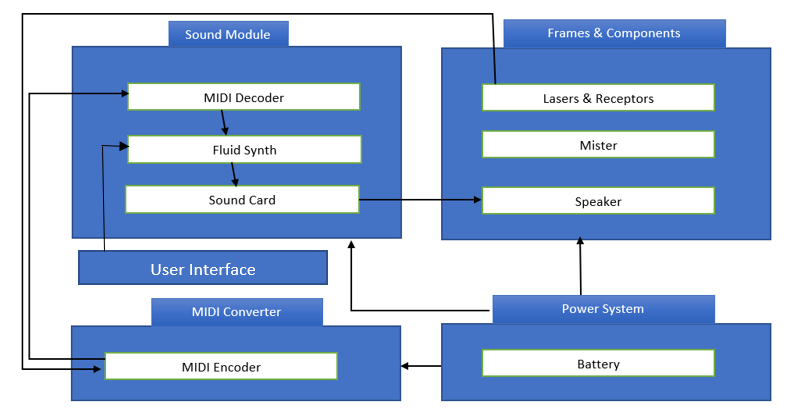
\includegraphics[width=0.90\textwidth]{images/data_flow}
 \caption{System architecture}
\end{figure}

\section{Roles \& Responsibilities}
The Team members for this project are: Ansih Yonian, Amir Dhunghana, Nik Purohit, Raul Jimenez, Rabinson Shrestha, and Roberto Torres. While there is no current sponsor for the project, we consider Professor McMurrough to be our client. Nik Purohit has taken on the role of being the Product Owner and will be responsible for finalizing the design of the system. As we begin implementation, the Product Owner will also ensure that the finished product meets the success criteria as outlined in the Project Charter. Roberto Torres is the Scrum Master for the project. The responsibilities of the scrum master include coordinating with all the team members and avoiding any scheduling conflicts, assigning the backlog tasks to team members, and generally planning out each sprint. As implementation of the system begins, the team will be divided into a hardware team and a software team. The hardware team will be responsible for the physical laser devices that generate the sounds as lasers are broken. The software team will be in charge of writing the scripts and code necessary for the software synthesizer to function and generate audio playback via MIDI inputs.

\section{Cost Proposal}
Based on previous laser harps that have been built, we have a range of our expected cost range. The cost range, as of September 22, 2019, will at a minimum of \$118.15. Based on previous projects we have analyzed we determined that their cost range is between \$118.55 and \$232.54 USD. 

\subsection{Preliminary Budget}
We listed several expenses below. We expect to not go over our allocated funding of \$800.00 USD. The expenses were broken into components, software licenses, and materials for the frame of the project.
\begin{table}[h]
\centering
\caption{Necessary Component Expense}
\begin{tabular}{ll}
Arduino Mega                & \$38.50 USD \\
Adafruit Music Maker Shield & \$34.95 USD \\
12V Power Supply            & \$10.00 USD \\
Laser diode                 & \$00.54 USD \\
Breadboard                  & \$05.90 USD 
\end{tabular}
\end{table}

\begin{table}[h]
\centering
\caption{Software Licenses}
\begin{tabular}{lll}
Blender             & GPL           & \$00.00 USD\\
AutoDesk AutoCAD    & Proprietery   & \$00.00 USD\\ 
\end{tabular}
\end{table}

Note: AutoDesk AutoCAD is provided by UTA IOT, thus their is no need to purchase a license.

\begin{table}[h]
\centering
\caption{Materials for Frame}
\begin{tabular}{ll}
Polyactic Acid  & \$00.05  USD \\
Nuts and Screws & \$09.99  USD \\
Wood            & \$17.95  USD
\end{tabular}
\end{table}

The pricing for the possible materials we will use has been listed above. This was a estimate with a margin of error. Thus costs could fluctuate above or below the expected budget costs.

\subsection{Current \& Pending Support}
As of September 22, 2019, we only have one source of funding. We do not expect the sources of funding to change. All of our funding for the project will be provided by the CSE department. The maximum amount they can provide to the project is approximately \$800.00 USD.
\section{Facilities \& Equipment}
We will need a 3D printer to print off part of our frame. This will require us to use either the 3D printer in the Central Library, or the 3D printer in Nedderman Hall Room 241. If later on we decide to use wood for some of our frame then we will need to borrow the band saw in Nedderman Hall Room 241. We will access to lab space when we assemble the laser harp. We will use lab space. Use of the laser cutter might be used to enhance the aesthetic of the laser harp. This will require us to borrow and use the laser cutter in Nedderman Hall Room 241. 

To test the laser harp we can conduct tests in the space where we will assemble the laser harp. Since the laser harp is stationary it will not require additional space to operate as it does not move. Additionally this space will need a power outlet as the laser harp will need to be powered electrically. We will require a space to hold the frame and harp. Other than the space needed to hold the laser harp, we will not need to use other space.

We will require a soldering iron for wiring components of the Laser harp. Thus we will need to borrow this from the lab space. Additionally, because of the audio that our instrument will be broadcasting we will require an environment that does not require earplugs, which can muffle sound. Thus the makerspace in Nedderman Hall Room 241 will suffice.

Additionally, we will require an mobile device capable of loading an APK or an iOS application which will be used to control the sounds produced by the laser harp. This will require us to have a mobile device in close proximity of the laser harp such that they can communicate with one another. Since all team members own a device capable of this, we will not be needing to purchase, borrow, or lease this equipment.

We do not intend to lease any equipment, nor do we expect to purchase any additional equipment or machines that were not specified in for this project. All machines and equipment is available to be borrowed in either the makerspace in Nedderman 241 or the UTA Central Library FabLab.
\section{Assumptions}
The following list contains critical assumptions related to the implementation and testing of the project.

\begin{itemize}
  \item The cost of completing the project will not exceed the amount of money designated by the CSE department.
  \item All the members of the team have some experience working with lasers, circuit boards, CAD software, Teensy controllers, and Raspberry Pi.
  \item The project will be complete and ready for testing within the 5th sprint cycle.
  \item The hardware equipment will not be tampered with by other CSE teams working in close proximity of our team.
  \item The workspace has ample amount of power and network connectivity.
  \item Team members have some basic knowledge about different musical notes.
\end{itemize}

\section{Constraints}
The following list contains key constraints related to the implementation and testing of the project.

\begin{itemize}
  \item The team has limited experience working with laser, circuits boards and android or IOS development.
  \item The total cost for development must not exceed \$800.
  \item Final prototype must be completed by May,2020.
  \item Schedule conflicts due to full time course load and work.
  \item The number of people working on the project is small.
  \item The final product should be portable and light weight.
\end{itemize}

\section{Risks}
The following high-level risk census contains identified project risks with the highest exposure.

\begin{table}[h]
\resizebox{\textwidth}{!}{
\begin{tabular}{|l|l|l|l|}
\hline
 \textbf{Risk description} & \textbf{Probability} & \textbf{Loss (days)} & \textbf{Exposure (days)} \\ \hline
 Scheduling conflict among team members  & 0.5 & 10 & 5 \\ \hline
 Wrong budget estimation  & 0.3 & 10 & 3 \\ \hline
 Internet access not available during testing  & 0.01 & 1 & 0.01 \\ \hline
 Misplacement of parts and circuit boards  & 0.10 & 2 & 0.2 \\ \hline
 Lack of availability of workspace & 0.1 & 3 & 0.3 \\ \hline
 Information gathering about lasers and circuits takes longer & 0.8 & 15 & 12 \\ \hline 
\end{tabular}}
\caption{Overview of highest exposure project risks} 
\end{table}

\section{Documentation \& Reporting}
\subsection{Major Documentation Deliverables}

\subsubsection{Project Charter}
The initial version of the Project Charter is the goal of the first sprint and will be delivered on October 1st 2019.
The Charter is expected to be updated mostly near the beginning of the project as the system requirements are finalized. Once this has been completed, items within the Charter will be checked after every sprint and any necessary updates will be added to the project backlog. The final version will be delivered at the end of the next semester, at the end of the project.

\subsubsection{System Requirements Specification}
The System Requirements Specification will be the goal of the second sprint and is expected to be delivered on the week of the 21st of October 2019. As we begin implementation, new requirements may become apparent or the feasibility of previous requirements may come into question. As design decisions are made to address these issues, the System Requirements Specification will be updated to reflect them.

\subsubsection{Architectural Design Specification}
The Architectural Design Specification will be the goal of the third sprint and is expected to be delivered on the week of the 11th of November 2019. As new design decisions are made, the Architectural Design Specification will be updated.

\subsubsection{Detailed Design Specification}
The Detailed Design Specification will be constantly looked at during the sprints and updated as implementation progresses. The final version is expected to be delivered at the end of the second semester.

\subsection{Recurring Sprint Items}

\subsubsection{Product Backlog}
System requirements will be broken up into discrete, manageable tasks that a single team member or pair of team members can address during a single sprint. These tasks will then be added to the Product Backlog. The Product Owner will prioritize the backlog and the Scrum master will assign the duties to individual members based on interests, skills, and which team they are participating in (hardware or software). The backlog will be stored and maintained in a GitHub Project page.

\subsubsection{Sprint Planning}
There will be eight sprints to be planned out by the Scrum Master in conjunction with the Product Owner.

\subsubsection{Sprint Goal}
The sprint goals will be decided by a team vote at a meeting prior to a sprint.

\subsubsection{Sprint Backlog}
The Product Owned will decide which items within the Product Backlog will be moved to the Sprint Backlog.

\subsubsection{Task Breakdown}
The Scrum Master and Product Owner will decide who is assigned which tasks. The decisions will be made based on interests, skills, and which team the member is a part of. Each team member will be responsible for maintaining their estimates for each of the tasks they are working on.

\subsubsection{Sprint Burn Down Charts}
Time spent on tasks will be self reported by the team members and a burn down chart will be generated by the scrum master.

\begin{figure}[h!]
    \centering
    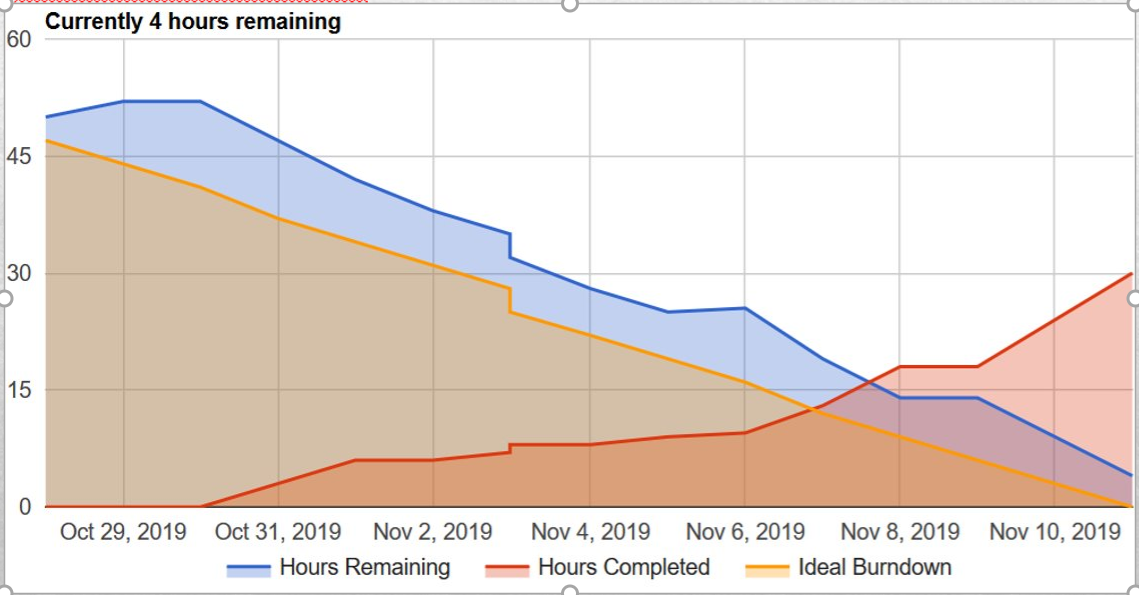
\includegraphics[width=0.5\textwidth]{images/temp0.PNG}
    \caption{Example sprint burn down chart}
\end{figure}

\subsubsection{Sprint Retrospective}
The Sprint Retrospective will take place immediately after a sprint and before the next sprint is planned. This will be an opportunity to raise any problems that members may have encoutered thoughout the sprint.

\subsubsection{Individual Status Reports}
Individual status reports will include a list of tasks a member is working on and their progress for each. Each member will be responsible for keeping their reports up to date.

\subsubsection{Engineering Notebooks}
The engineering notebooks will be signed periodically during stand-ups. Anyone within the team with knowledge of what is on a given notebook will be able to sign the notebook as a witness.

\subsection{Closeout Materials}

\subsubsection{System Prototype}
Our final System Prototype will be tested by someone who knows how to play a musical instrument for a final demonstration for the class.

\subsubsection{Project Poster}
The Project Poster will be depict the process we underwent to create the final product and include a depiction of the final prototype.

\subsubsection{Web Page}
Our project will have an informational webpage that will include links to the source code and the demo video.

\subsubsection{Demo Video}
The demo video will show a demonstration of the laser instrument being played as well as a step-by-step guide of how to configure it using the mobile app.

\subsubsection{Source Code}
The source code will be maintained on a GitHub repository. The resulting application code and schematics will be made available to the public under the GNU General Public License.

\subsubsection{Source Code Documentation}
Doxygen will be used to generate the source code documentation which will be published on the project web page.

\subsubsection{Hardware Schematics}
Hardware Schematics for the laser devices and the sound producing device will be made available throught the project web page.

\subsubsection{User Manual}
A user manual and set up video will be made available through the project web page.

\newpage

%%% References
\bibliographystyle{plain}
\bibliographystyle{reference/IEEEtran_custom}
\bibliography{reference/refs}{}

\end{document}
